%!TEX root = bachelor.tex
\chapter{Theoretische Grundlagen}
\label{ch:theory}

Rechtshändiges Koordinatensystem...
\section{Kegel}
\label{s:cone}

\begin{figure}[!htb]
	\centering
	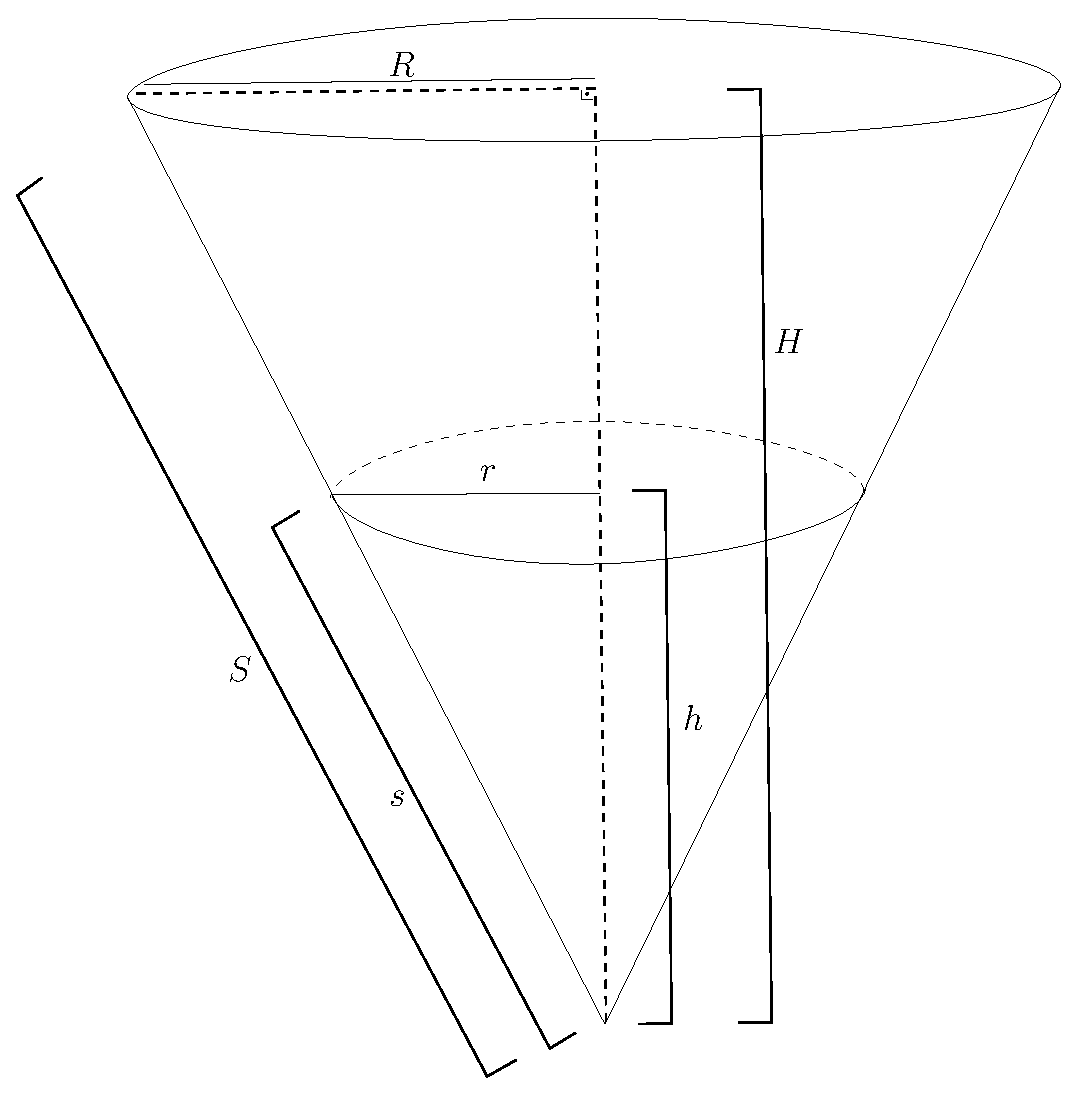
\includegraphics[scale=.5]{images/fullCone3.eps}
	\caption{Gerader Kreiskegel}
	\label{fig:cone}
\end{figure}

Kreisgrundläche mit Radius 


normaler Kegel Spitze $S(0,0,0)$
\begin{equation}
\begin{aligned}
x &= \frac{u}{h} R~cos \theta \\
y &= u \\
z &= \frac{u}{h} R~sin \theta
\end{aligned}
\end{equation}
mit $u\in [0, H]$ und $\theta \in [0, 2\pi)$


\begin{figure}[!htb]
	\centering
	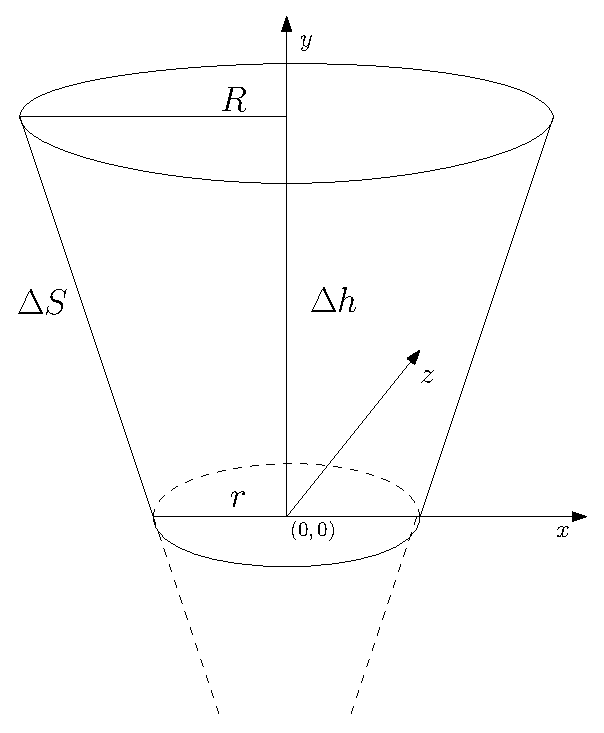
\includegraphics[scale=.7]{images/coneFrustum.eps}
	\caption{Kegelstumpf}
	\label{fig:coneFrustum}
\end{figure}


\begin{equation}
\begin{aligned}
x &= (r + \frac{u}{h} (R - r))~cos \theta \\
y &= u \\
z &= (r + \frac{u}{h} (R - r))~sin \theta
\end{aligned}
\end{equation}
mit $u\in [0, \Delta H]$ und $\theta \in [0, 2\pi)$


\begin{figure}[!htb]
	\centering
	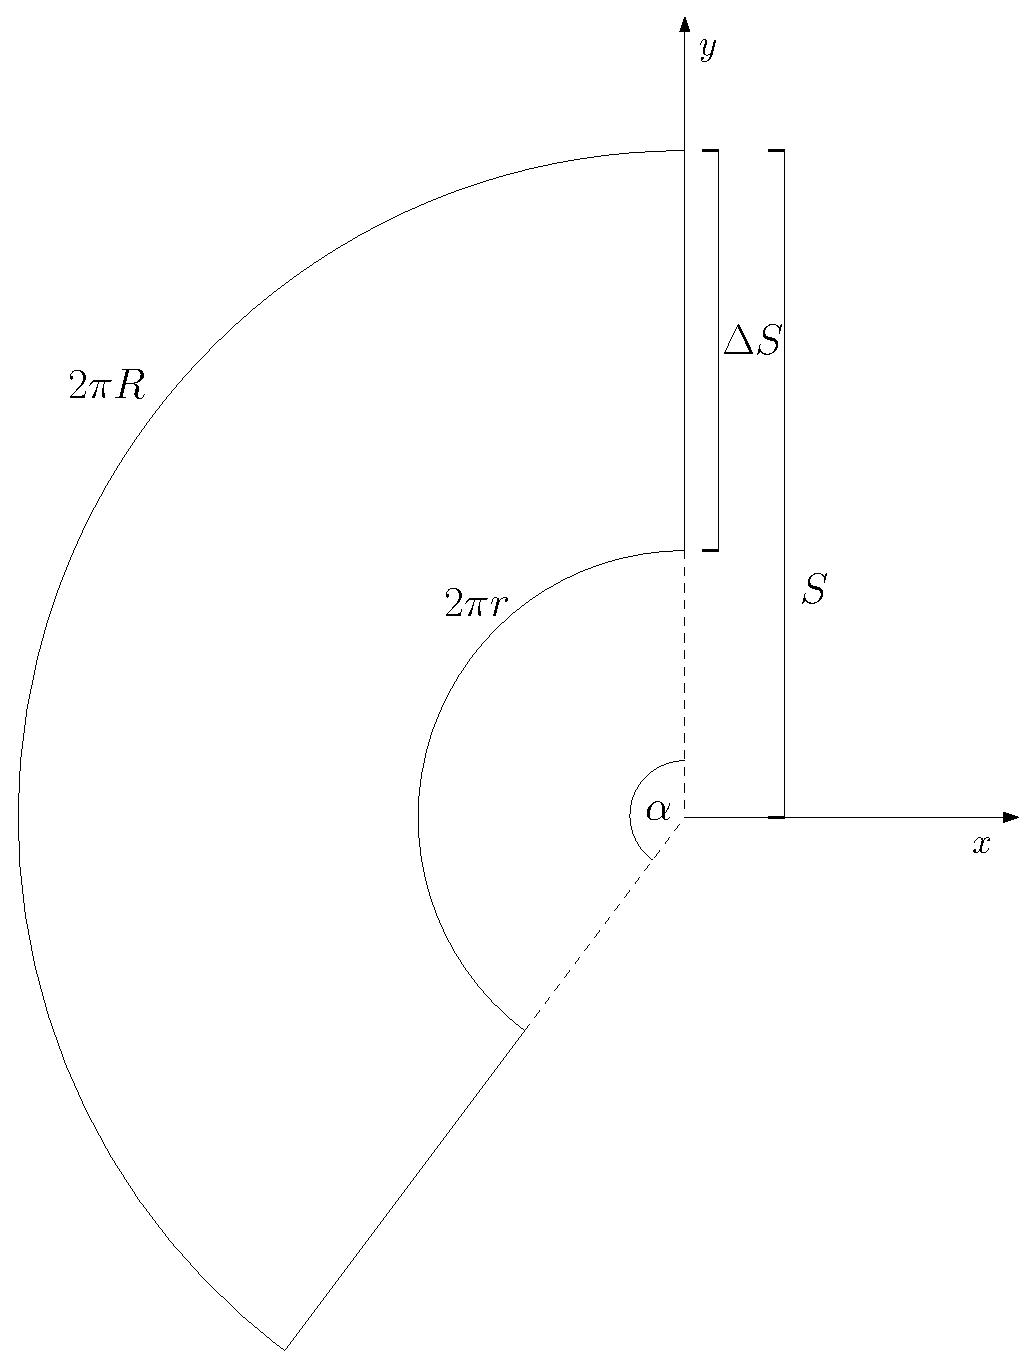
\includegraphics[scale=.4]{images/coneLateral.eps}
	\caption{Kegelmantelfläche}
	\label{fig:coneLateral}
\end{figure}



\begin{equation}
\begin{aligned}
x &= -(s + \lambda (S-s)) ~sin \phi \\
y &= (s + \lambda (S-s)) ~cos \phi
\end{aligned}
\end{equation}
mit $\lambda \in [0, 1]$ und $\phi \in [0, \alpha]$




Sei $\mathcal{R}(y) := r + \frac{y}{h} (R - r)$, $\Phi(x,y,z) := \atant\left(\frac{z}{d(y)}, \frac{x}{d(y)}\right)$, $\mathcal{S}(y) := s + \frac{y}{\Delta H} (S-s)$
\begin{equation}
\begin{aligned}
\Psi \colon [r,R] \times [0, \Delta H] \times [r,R] &\to [s,S] \times [s,S]\\
(x,y,z) &\mapsto \left(-\mathcal{S}(y)\sin \Phi(x,y,z), \mathcal{S}(y)\cos\Phi(x,y,z)\right) 
\end{aligned}
\end{equation}

Sei $\mathcal{R}(y) := r + \frac{y}{h} (R - r)$, $\Phi(x,y,z) := \atant\left(\frac{z}{d(y)}, \frac{x}{d(y)}\right)$, $\mathcal{S}(y) := s + \frac{y}{\Delta H} (S-s)$
\begin{equation}
\begin{aligned}
\Psi^{-1} \colon  [s,S] &\to [r,R] \times [0, \Delta H] \times [r,R]\times [s,S]\\
(x,y,z) &\mapsto \left(-\mathcal{S}(y)\sin \Phi(x,y,z), \mathcal{S}(y)\cos\Phi(x,y,z)\right) 
\end{aligned}
\end{equation}




\newpage

Gerader Kreiskegel
kamerakalibrierung

projektionsmatrix
(homogene Koordinaten????)
SVD, QR, LSQ?

kegel koordianten

kegel mantelfläche

kegel abbildungen

Hough?

Paremterschätzung Ransac. anzahl interationen

ellipse distanz mit transformationen die nötig sind

Hauptachsentransformation

schnittpunkt linie ellipse


Kantendetektion (canny sobel)


evtl noch am ende delaunay

deformable templates